The plotting system is implemented using ScottPlot\citep{scottPlot}, a plotting library for .NET\@.

The functionality is exposed to the user through 3 built-in functions: \textit{plot}, \textit{plotFunc} and 
\textit{plotFuncs}.

\paragraph{\textit{plot}} takes in a record of configuration options of the following type:

\begin{minted}{fsharp}
    type PlotConfig = {
        title: string,
        x: [float],
        y: [float],
        ptype: "bar" | "scatter" | "signal",
    }
\end{minted}

The resulting plot is then displayed in a separate window based on these configuration options.

Here are some examples of the \textit{plot} function in use:

\begin{minted}{fsharp}
let x = [1..10] : [float]
let y = map(x, (x) -> x^2)
let data = {
    title = "Example Plot",
    x = x,
    y = y,
    ptype = "scatter"
}
plot(data)
\end{minted}

Image~\ref{fig:scatter-plot} shows the resulting plot.

\begin{figure}[H]
    \centering
    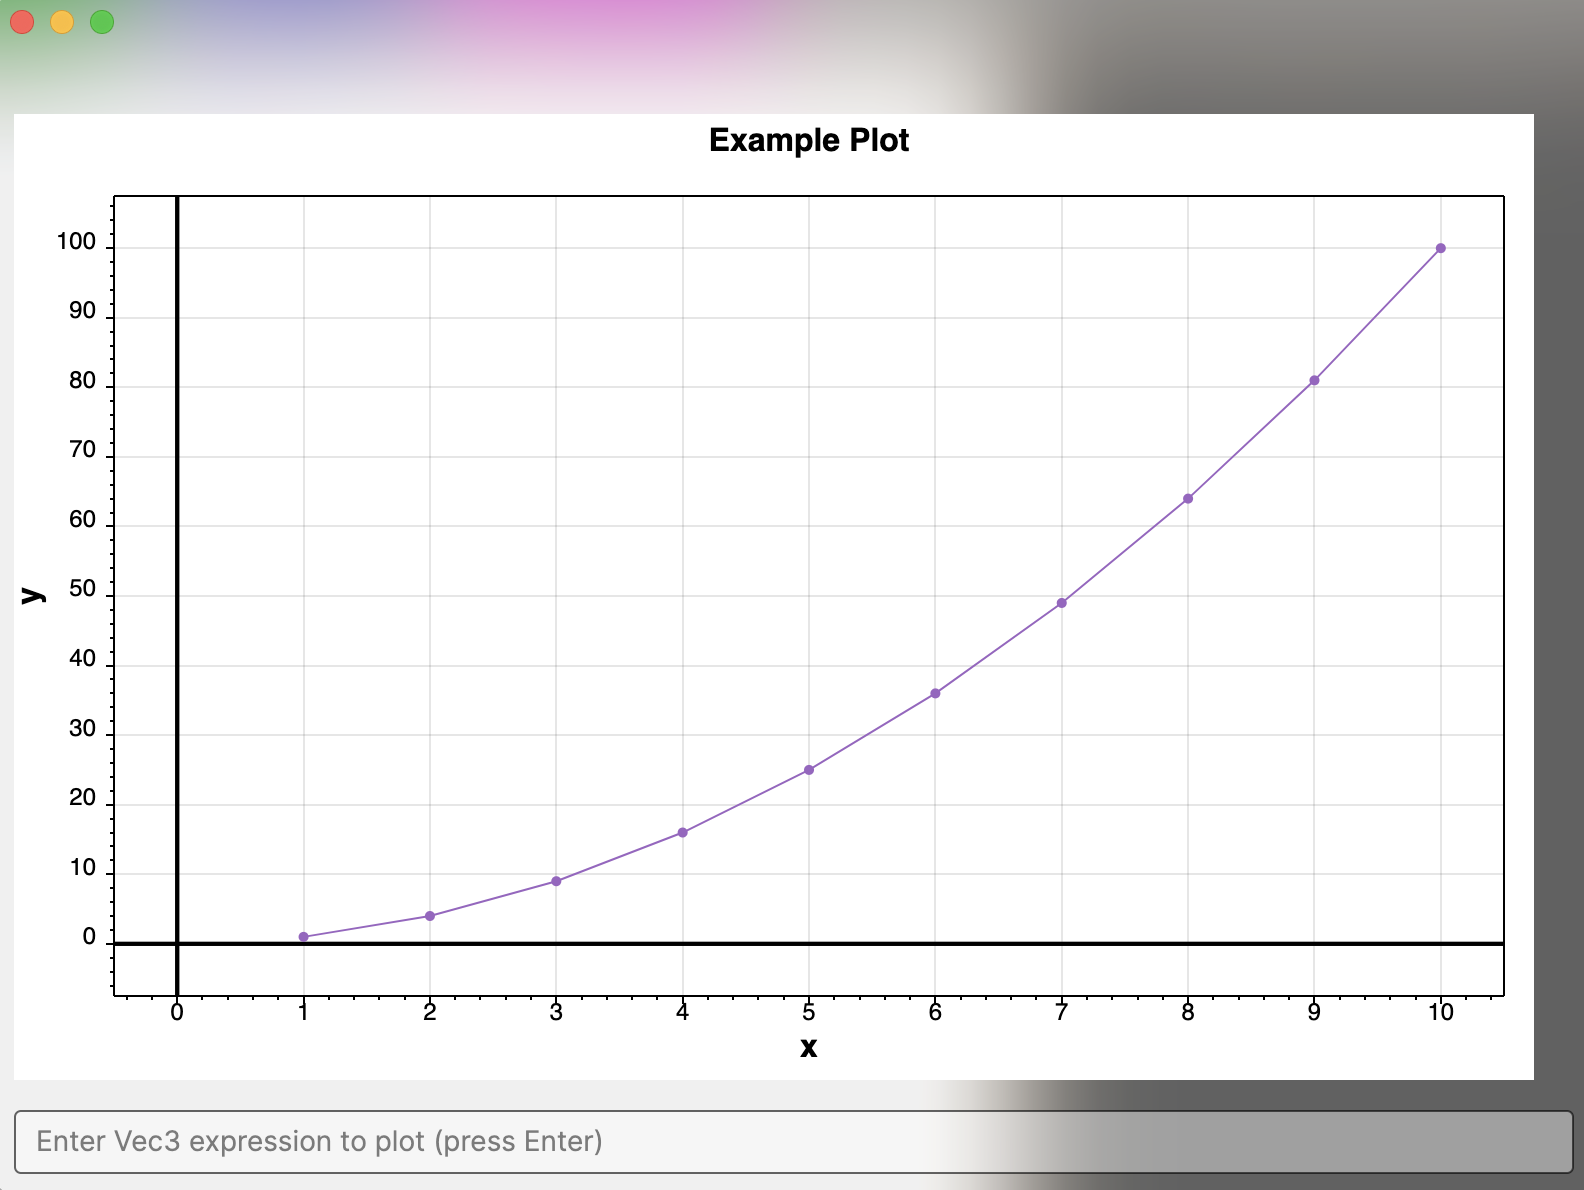
\includegraphics[width=0.8\textwidth]{assets/scatterPlot}
    \caption{Scatter plot}\label{fig:scatter-plot}
\end{figure}

The \textit{ptype} option allows for the user to specify the type of plot, with the options being \textit{bar},
\textit{scatter} and \textit{signal}.

The \textit{bar} type is useful for visualising data, the \textit{scatter} type is useful for plotting functions and
the \textit{signal} type is useful for plotting signals.
An example of a bar plot is shown in image~\ref{fig:bar-plot}.

\begin{figure}[H]
    \centering
    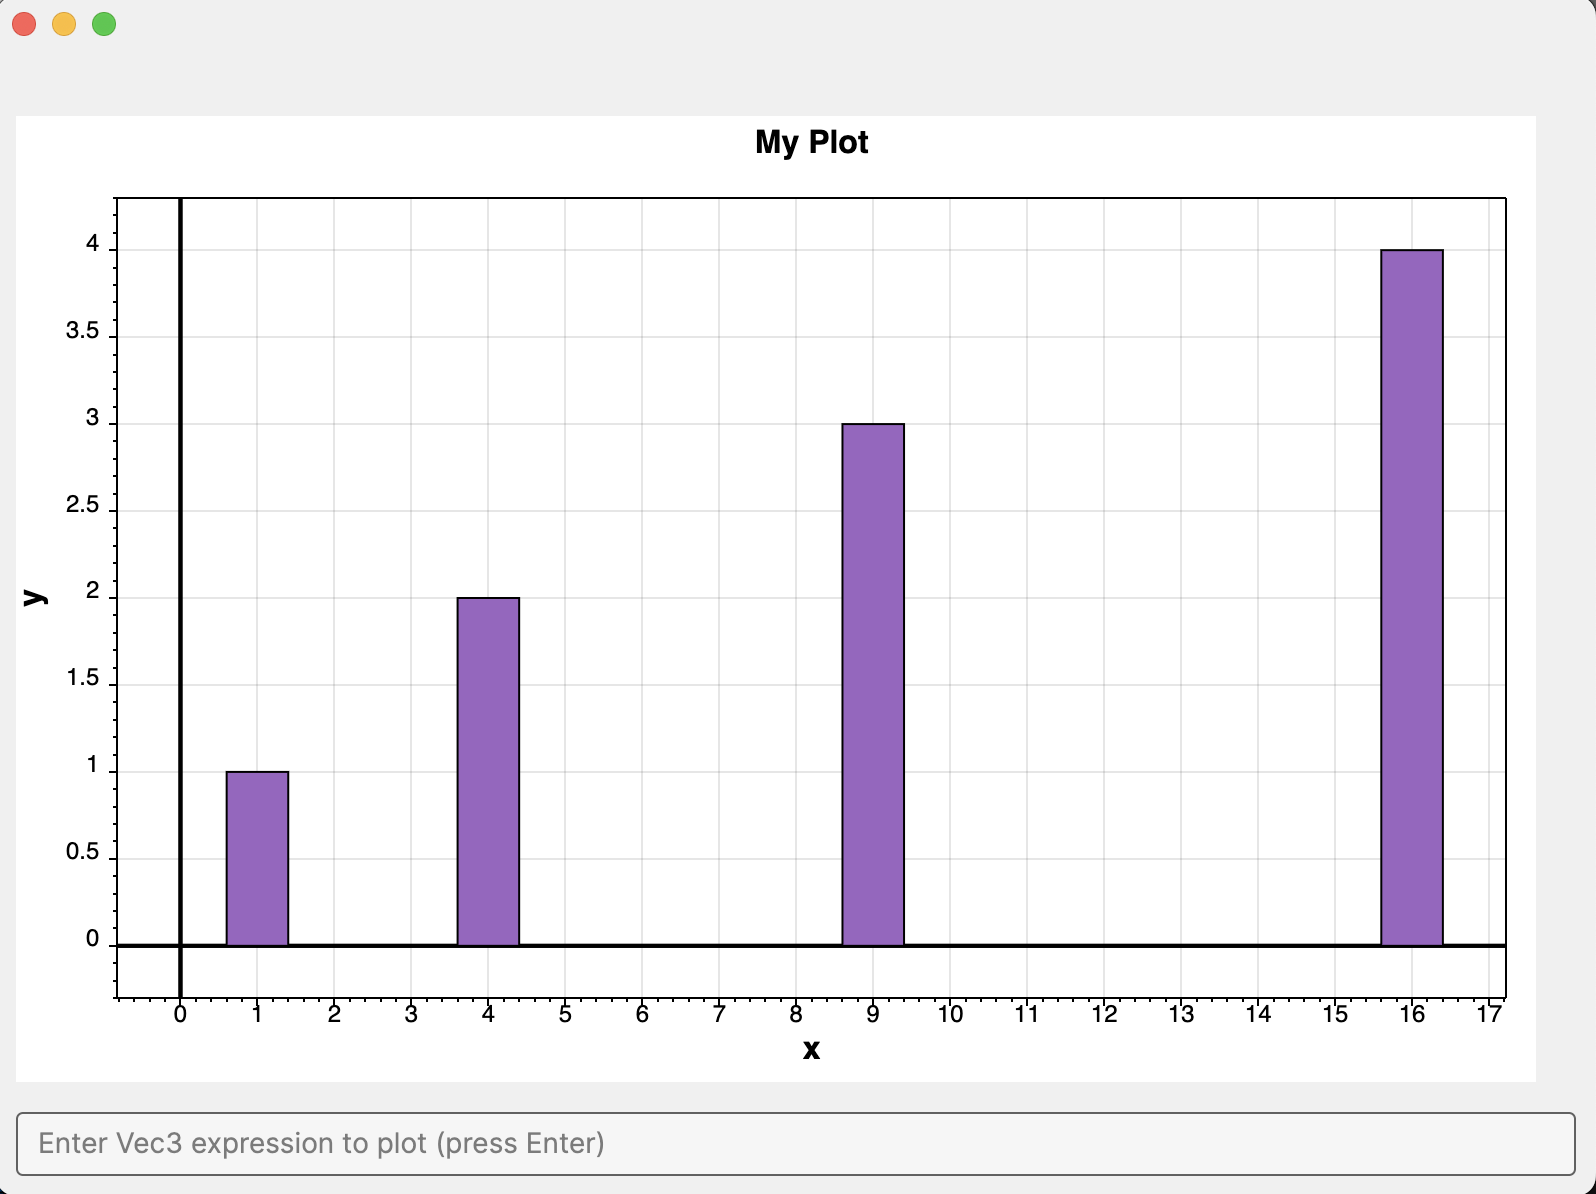
\includegraphics[width=0.8\textwidth]{assets/barChart}
    \caption{Bar plot}\label{fig:bar-plot}
\end{figure}

\paragraph{The \textit{plotFunc}} function takes in a string title and a pure function of type \textit{float -> float}.
The function is then plotted on the graph with an infinite range of x values.
Optionally, the user can also specify two more float values, \textit{start} and \textit{end}, in which case the 
integral of the function is calculated and displayed on the graph.

For example, given the following snippet:

\begin{minted}{fsharp}
let polynomial = (x) -> x^2 + 2.0 * x + 1.0
plotFunc("Polynomial", polynomial)
\end{minted}

Image~\ref{fig:polynomial-plot} shows the resulting plot.

\begin{figure}[H]
    \centering
    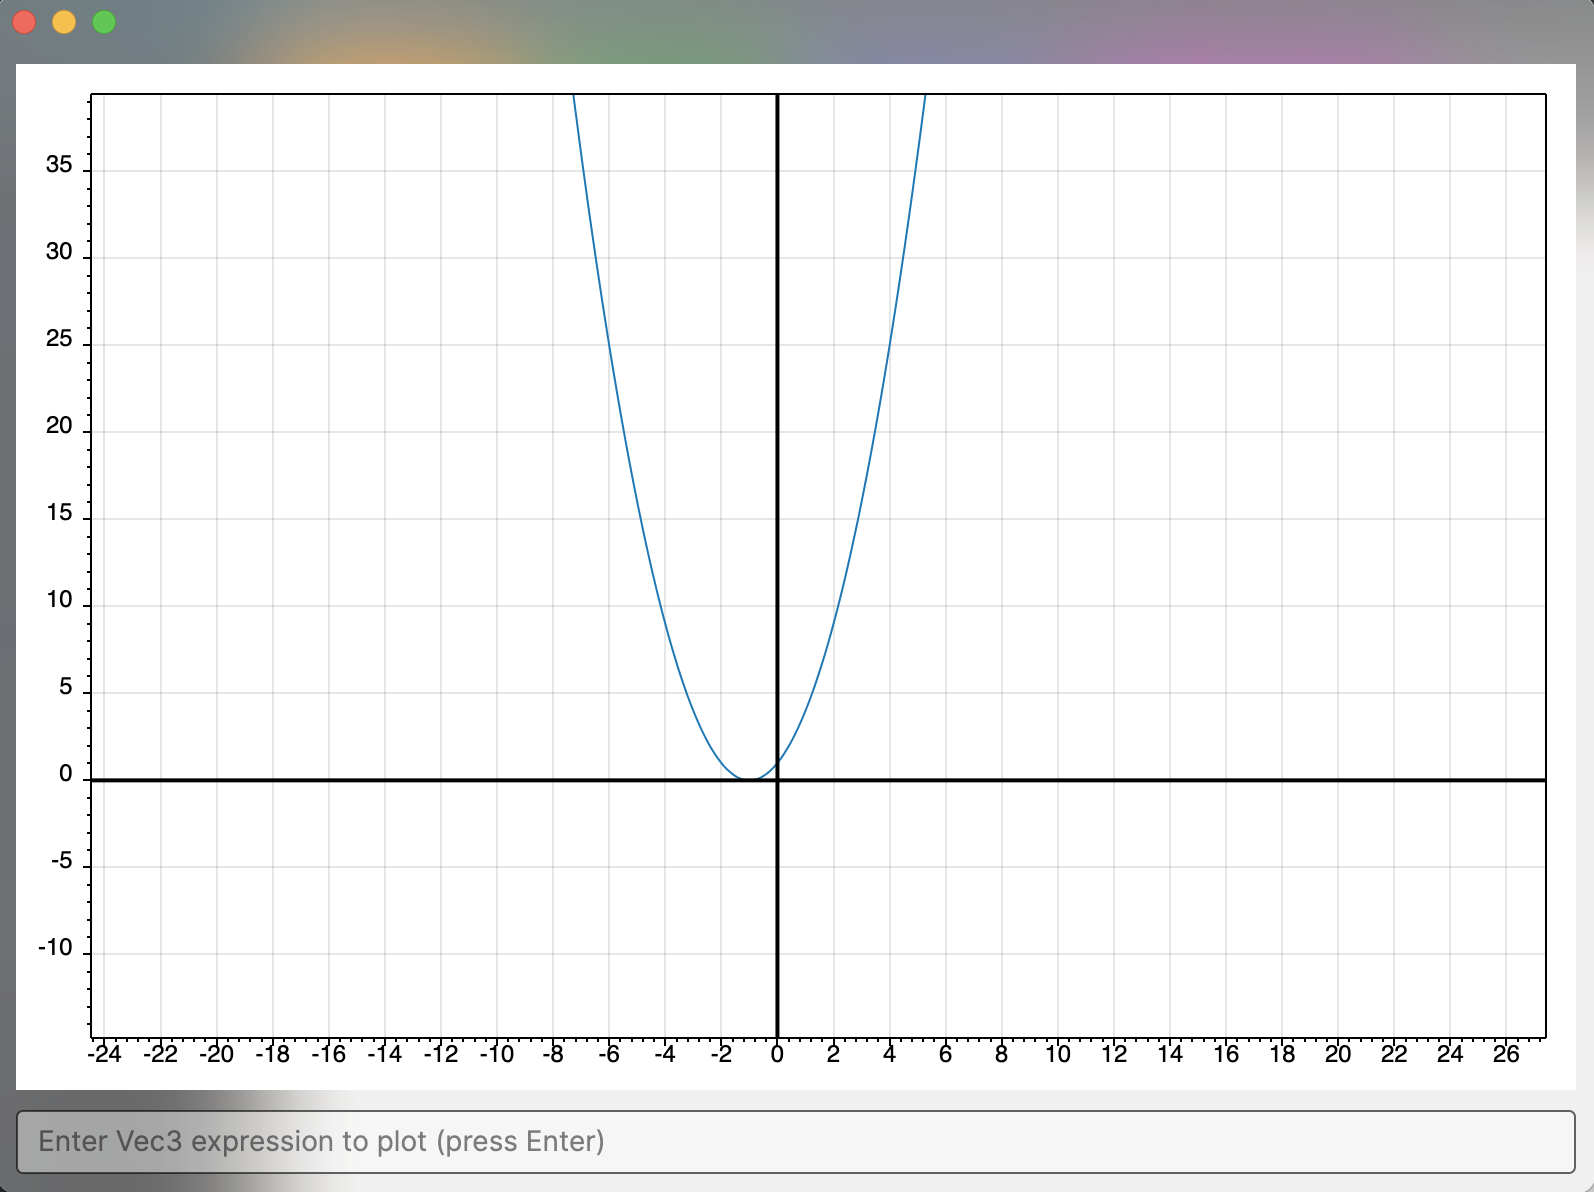
\includegraphics[width=0.8\textwidth]{assets/polynomialPlot}
    \caption{Polynomial plot}\label{fig:polynomial-plot}
\end{figure}

A point of interest is that for both the \textit{plotFunc} and \textit{plotFuncs} functions, a legend is provided 
with a textual representation of the function being plotted.
This is particularly useful when plotting multiple functions on the same graph, or when dynamically plotting 
functions (or their derivatives/integrals) based on user input.

\paragraph{The \textit{plotFuncs}} function takes in a string title and a list of pure functions of type 
\textit{float -> float}.
This allows for multiple plots to be placed on the same window, which we felt was valuable for comparing functions 
or plotting derivatives.

For example, given the following snippet:

\begin{minted}{fsharp}
let polynomial = (x) -> x^2 + 2.0 * x + 1.0
let derivate = differentiate(polynomial) // find the derivative of the polynomial
let integrand = integrate(polynomial) // find the integral of the polynomial
let tangentFunc = tangentFunc(polynomial, 2.0) // find the tangent function at x = 2.0

plotFuncs("Polynomial", [polynomial, derivate, integrand, tangentFunc])
\end{minted}

Image~\ref{fig:multiple-plots} shows the resulting plot.

\begin{figure}[H]
    \centering
    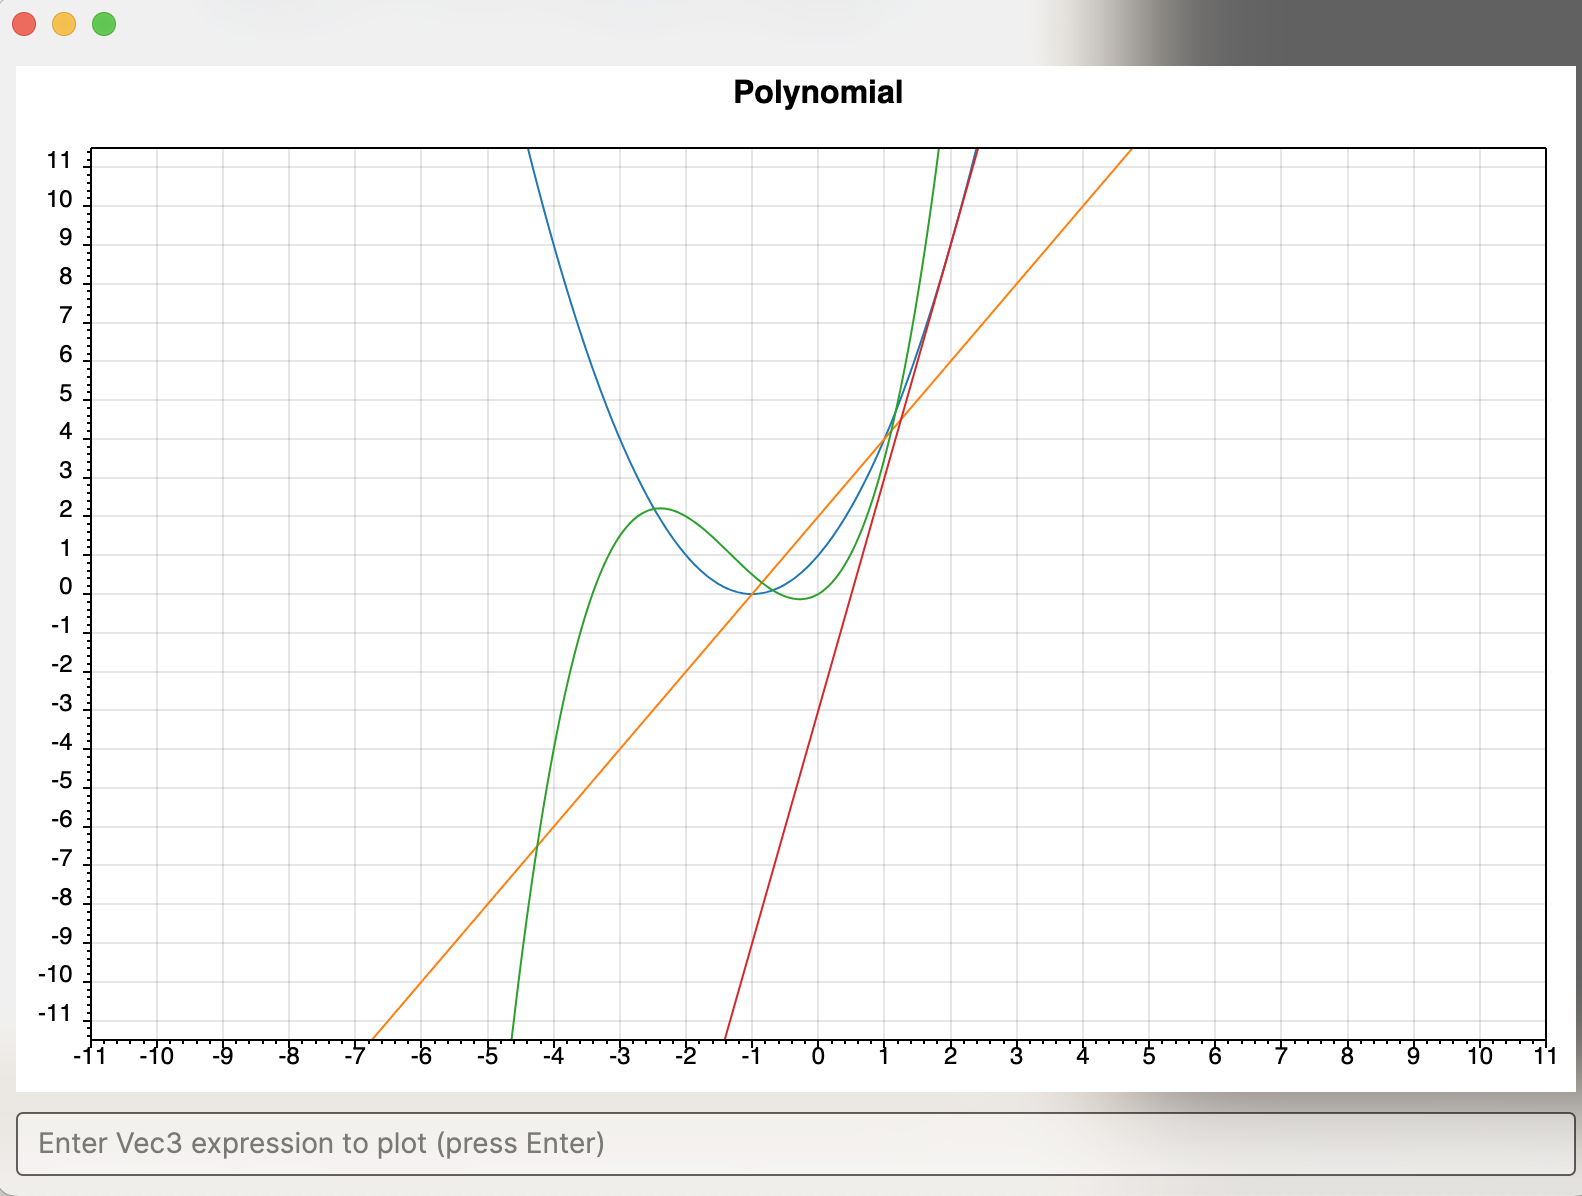
\includegraphics[width=0.8\textwidth]{assets/multiplePlots}
    \caption{Multiple plots}\label{fig:multiple-plots}
\end{figure}

The plots are very interactive, with the user being able to zoom in and out, move around and adjust the axes as
desired.

The plot windows also have an input at the bottom, which allows for the user to input a function and have it plotted
on command\ref{fig:plot-input}.
This is useful for quick visualisation of functions, and allows for a more interactive experience.
Note that variable resolution is performed on the input, allowing for the user to use variables defined in the
program in the input.
Additionally, the legend updates dynamically.

\begin{figure}[H]
    \centering
    
\includegraphics[width=0.8\textwidth]{assets/plotInput}
    
\includegraphics[width=0.8\textwidth]{assets/plotInput2}
    \caption{Plot input}\label{fig:plot-input}
\end{figure}